\documentclass{beamer}
\usepackage{graphicx, tikz, multicol, amsmath, amssymb, amsfonts} % Required for inserting images
\usepackage{multirow}
\usepackage{ tikz-imagelabels} % Required for inserting images
\usepackage{pifont}
\usetheme{Madrid}
\usecolortheme{dove}
\usepackage{hyperref}
\hypersetup{
    colorlinks=true,
    linkcolor=white,
    filecolor=magenta,      
    urlcolor=red,
    pdftitle={Overleaf Example},
    pdfpagemode=FullScreen,
    }

\urlstyle{same}


%\usepackage[backend=bibtex, style=numeric, sorting=none, locallabelwidth]{biblatex}
%\bibliography{reference.bib}
%\usefonttheme{structurebold}
%\usefonttheme{serif}
%\usepackage[dvipsnames]{xcolor}
\usefonttheme{professionalfonts}
\usepackage{xcolor}

\usepackage{tikz}
\usepackage{tikz-imagelabels}
\usepackage{tcolorbox}
\setbeamertemplate{frametitle}[default][center]
\definecolor{uvablue}{RGB}{35,45,75}
\definecolor{uvaorange}{RGB}{229,114,0}
\definecolor{UniBlue}{RGB}{83,121,170}
\definecolor{forestgreen}{RGB}{0,128,0}
\definecolor{bronze}{rgb}{0.8, 0.5, 0.2}
\definecolor{purple}{RGB}{128,0,128}
\definecolor{maroon}{RGB}{184,15,10}
\definecolor{grey}{RGB}{128,128,128}
\definecolor{bondiblue}{rgb}{0.0, 0.58, 0.71}
\definecolor{gold}{RGB}{160,116,10}
\setbeamercolor{title}{fg=UniBlue} %bg=white}
\setbeamercolor{frametitle}{fg=UniBlue,}% nbg=UniBlue}
\setbeamercolor{framesubtitle}{fg=black, bg =UniBlue}
\setbeamercolor{palette primary}{bg=UniBlue,fg=white}
\setbeamercolor{palette secondary}{bg=UniBlue, fg=white}
\setbeamercolor{palette tertiary}{bg=UniBlue,fg=white}
\setbeamercolor{palette quaternary}{bg=UniBlue,fg=white}
%\setbeamercolor{structure}{fg=UniBlue}
\setbeamercolor{footline}{fg=uvablue}

\imagelabelset{
%coarse grid color = red,
%fine grid color = gray,
%image label font = \sffamily\bfseries\small,
%image label distance = 2mm,
%image label back = black,
%image label text = white,
coordinate label font = \sffamily\bfseries\tiny,
coordinate label distance = 1mm,
coordinate label back = white ,
coordinate label text = uvaorange,
annotation font = \normalfont\tiny,
%arrow distance = 1.5mm,
%border thickness = 0.6pt,
%arrow thickness = 0.4pt,
%tip size = 1.2mm,
%outer dist = 0.5cm,
}
\bibliography{reference.bib}
\title[SIDM]{Search For Self-Interacting Dark Matter \\ With Displaced Lepton Jets}
\subtitle{Lepton Jet Reconstruction Efficiency}
%\institute[UVA]{University of Virginia}
\author[Maria Jose]{\scriptsize Sam Bright-Thonney$^0$, Xuan Chen$^0$, Jose Monroy$^0$, Julia Thom$^0$, Valentina Dutta$^0$, Kyungmin Park$^1$, Manfred Paulini$^1$, Bo Jayatilaka$^2$, Murtaza Safdari$^2$, Sunil Dogra$^3$, Dongyub Lee$^3$, Chang-Seong Moon$^3$, Andre Frankenthal$^4$, Gail Hanson$^5$, \\Joaquin Siado Castaneda$^6$, Daniel Claes$^6$, Grace Haza$^6$, Bryan Cardwell$^7$, \textbf{Maria Jose}$^7$,\\ Reshma Menon R$^7$, Chris Neu$^7$, Carter Patten$^7$, Allie Hall$^{2,8}$}
\date[\today]{\today}
\logo{%
  
  
\includegraphics[width=1cm,height=1cm,keepaspectratio]{../UniversityLogos/CMSlogo.png}%
   \hspace{\dimexpr\paperwidth -2cm-2.5pt}%
  \vspace{\dimexpr\paperwidth -2cm-2.5pt}%
  
\includegraphics[width=1cm,height=1cm,keepaspectratio]{../UniversityLogos/rotunda.jpg}%
 
}
\titlegraphic{
\includegraphics[width =12cm, height =1 cm]{../UniversityLogos/logos.png}}

%\titlegraphic{
\includegraphics[width=1cm,height=1cm]{cornell.png} 
%
\includegraphics[width = 1cm, height= 1cm]{cmu.png}
%
\includegraphics[width = 1cm, height =1cm]{fnal.png}
%
\includegraphics[width = 1cm, height =1cm]{knu.jpeg}
%
\includegraphics[width = 1cm, height =1cm]{princeton.png}
%
\includegraphics[width = 1cm, height =1cm]{ucriverside.png}
%
\includegraphics[width = 1cm, height =1cm]{unebraska.jpg}
%
\includegraphics[width =1cm, height =1cm]{uvalogo.png}
%
\includegraphics[width = 1cm, height =1cm]{United_States_Naval_Academy.png}}
%


\begin{document}
{
\setbeamertemplate{logo}{ 
  
\includegraphics[width=1cm,height=1cm,keepaspectratio]{../UniversityLogos/CMSlogo.png}%
   \hspace{\dimexpr\paperwidth -1.75cm-2.5pt}%
  \vspace{\dimexpr\paperwidth -1.75cm-2.5pt}%
  
\includegraphics[width=1cm,height=1cm,keepaspectratio]{../UniversityLogos/lpcdm_logo.png}
  }
\begin{frame}
\maketitle
\end{frame}
}

%\begin{frame}{Why Self Interacting Dark Matter?}
%\begin{itemize}
%
%   \item CDM model of cold, collision-less dark matter explains things at a large length scale but fails to explain small-scale issues.
%    \item Mass distributions in galaxy clusters reveal dark matter density cores in the inner regions in contrast to cusps predicted by CDM.
%      \item This issue could be resolved if dark matter has self-interactions. It is consistent with observations at a larger scale, too.
%\end{itemize}
%
%\end{frame}
\begin{frame}{Outline}
\begin{enumerate}

    \item SIDM Model
    \item Lepton Jets (LJs)
    \item LJ Reconstruction Efficiency Definition
    \item Lepton Collimation
    \item $e\gamma$ LJ Reconstruction Efficiency
    \item $\mu$ LJ Reconstruction Efficiency
    \item Conclusion

\end{enumerate}
\end{frame}
\begin{frame}{Self Interacting Dark Matter (SIDM) Model }
\vspace{-0.2cm}
\begin{columns}
\begin{column}{.2\textwidth}
\begin{center}
    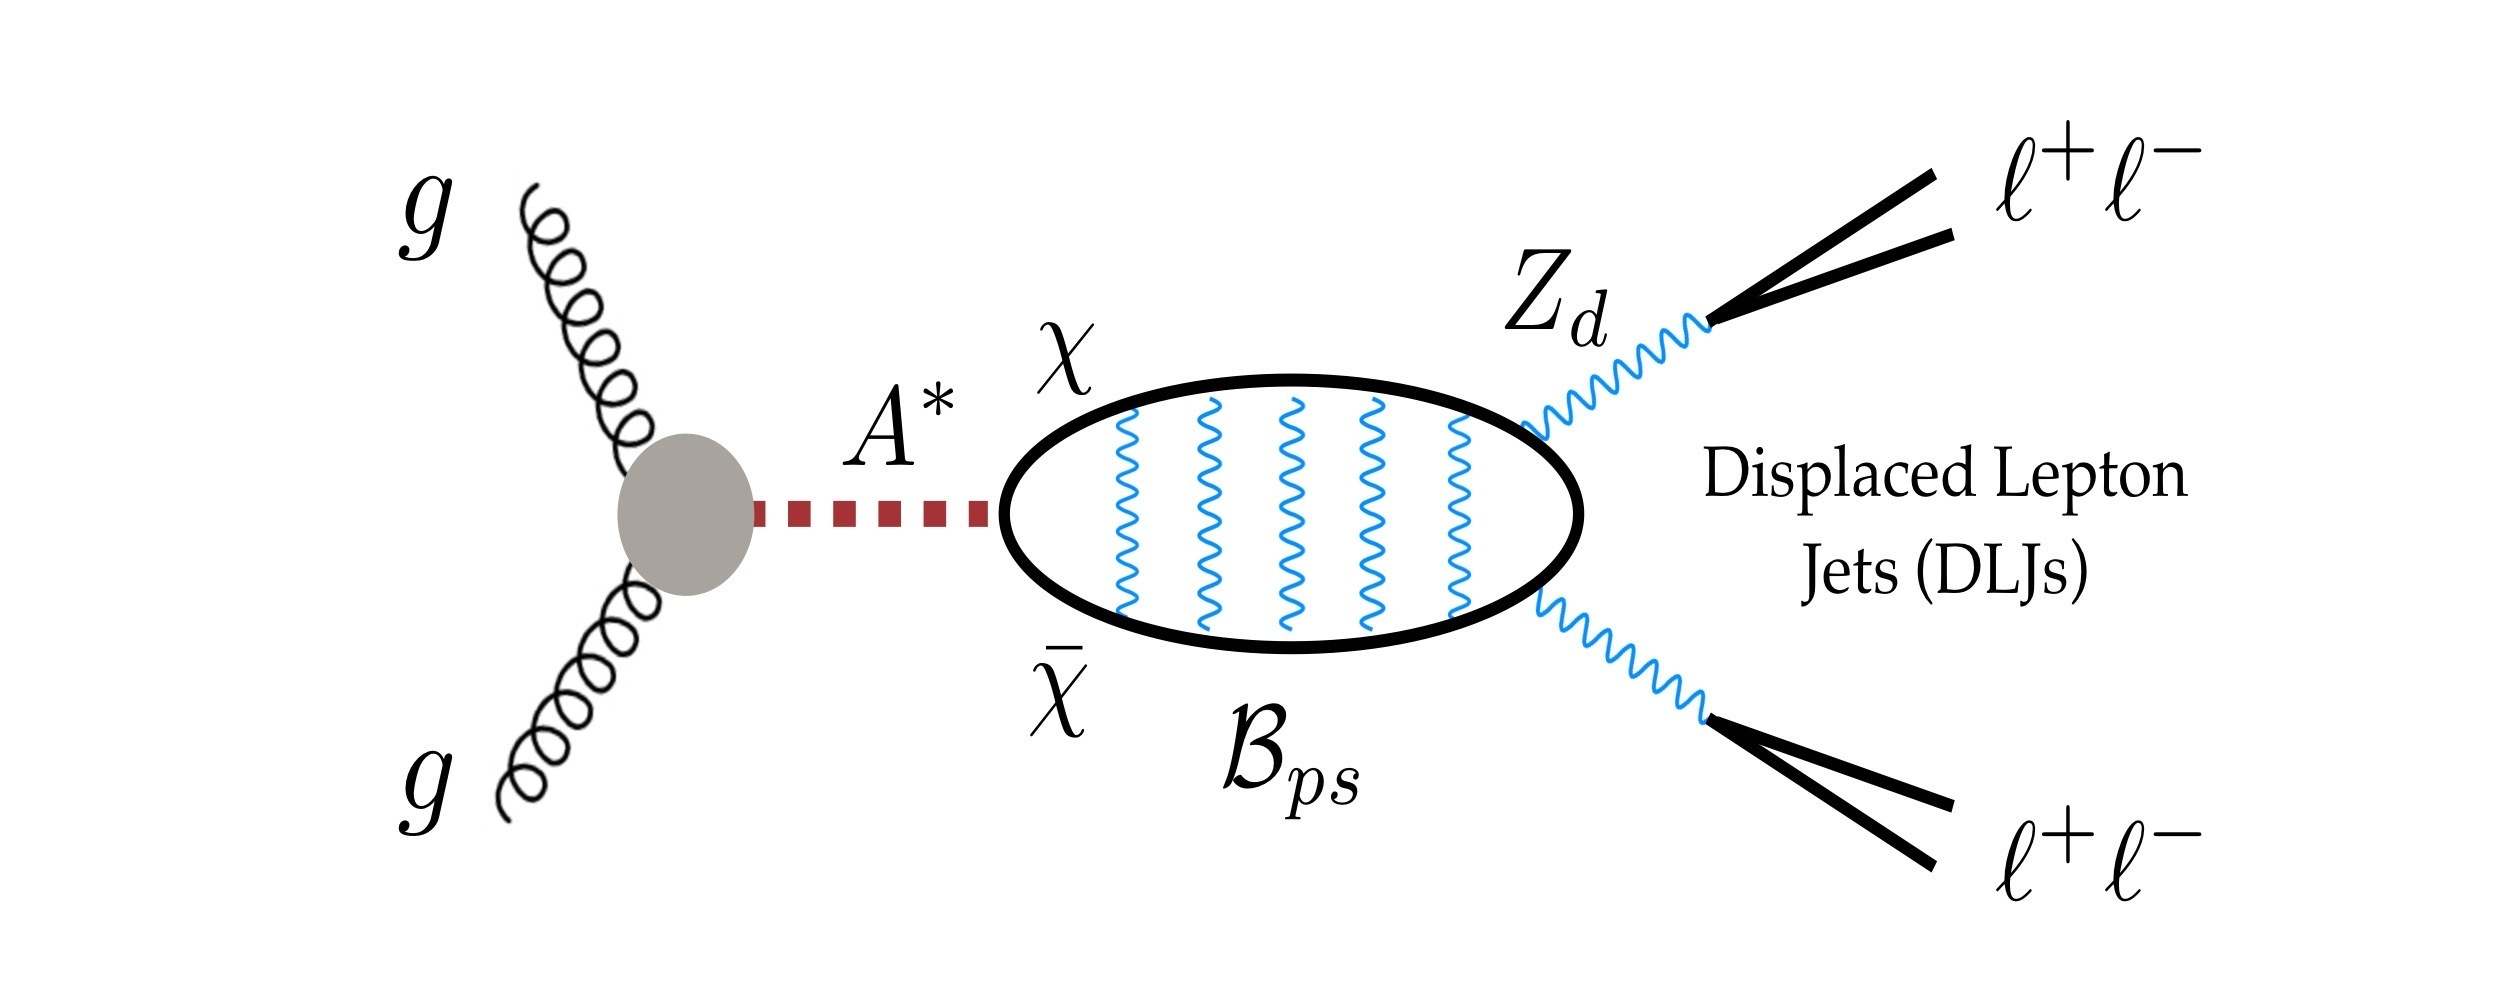
\includegraphics[width =3.5 cm, height = 2.5 cm]{FeyDia.jpg}\\
    %\tiny{Reprinted from \cite{sidm_}}
\end{center}
\end{column}
\hspace{.5cm}
\begin{column}{.7\textwidth}
\begin{tcolorbox}[colback=uvaorange!5!white,colframe=uvaorange]
\begin{enumerate}
    \item Light \textbf{$Z_d$} $\rightarrow$ \textcolor{red}{Boosted $Z_d$}
       \item Small $Z_d$ - SM Coupling \\ $\rightarrow$ \textcolor{red}{Long-Lived $Z_d$}
       \item Displaced decays of boosted $Z_d$ $\rightarrow$ \textcolor{red}{Displaced, collimated leptons }(\textcolor{forestgreen}{Displaced Lepton Jets (LJs)})
\end{enumerate}
   
\end{tcolorbox}
\end{column}
\end{columns}


\begin{columns}

\begin{column}{.64\textwidth}
\textbf{\textcolor{UniBlue}{Free Parameters:}}
    \begin{itemize}
     \item Bound state mass ($m_B$)
     \item Dark photon mass ($m_{Z_d}$)
     \item Kinetic mixing between $Z_d$ and SM, $\epsilon$
     \end{itemize}
 \textbf{\textcolor{UniBlue}{Signal:}}
 \begin{itemize}
     \item   $m_B$ $\epsilon$ [100, 150, 200, 500, 800, 1000] GeV
     \item $m_{Z_d}$ $\epsilon$ [0.25, 1.2, 5] GeV
     \item $Z_d$ $L_{xy}$ $\epsilon$ [0.3, 3, 30, 150, 300] cm
 \end{itemize}
\end{column}
\begin{column}{.36\textwidth}
     \textbf{\textcolor{UniBlue}{Final states} :  $2\mu2e$ or $4\mu$}\\
%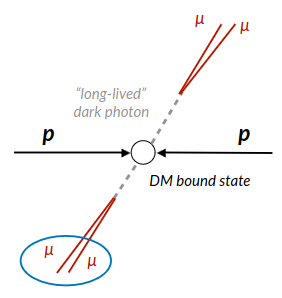
\includegraphics[width =4cm, height = 4cm]{lj.png}
\begin{annotationimage}{width=4cm, height=4cm}{lj.png}
%\draw[coordinate label  = {$Z_d \rightarrow ee$ at (0.5, -.05)}];
\draw[coordinate label  = {\textcolor{bondiblue}{LJ}  at (0.5, 0.1)}];
\draw[coordinate label  = {\textcolor{maroon}{$\mu/e$}  at (0.9, 0.9)}];
\draw[coordinate label  = {\textcolor{maroon}{$\mu/e$}  at (0.65, 0.95)}];
\end{annotationimage}
\end{column}
\end{columns}   
    
\end{frame}
\begin{frame}{Lepton Jets (LJs)}
\begin{itemize}
   \item Group of collimated leptons in a tight cone.
   \item We apply anti- $k_T$ clustering ($\Delta$R = 0.4) to \textbf{PF $e$, PF $\gamma$, PF $\mu$} and \textbf{DSA $\mu$}.
\end{itemize}
\begin{columns}
\begin{column}{.32\textwidth}
\textbf{\textcolor{UniBlue}{Conditions to reconstruct an LJ:}}\\
\begin{itemize}
    \item $\lvert \eta \rvert<$ 2.4
    \item $p_T>$ 30 GeV
    \item $\sum{Q_{\mu}}=$0\\
    (to prevent b-quark
    cascade decays)
\end{itemize}
\textbf{\textcolor{UniBlue}{Categories of LJs:}}\\
\begin{itemize}
    \item $e\gamma$ ($N_{\mu}=$0)
    \item $\mu$ ($N_{\mu}>=$1)
\end{itemize}
\end{column}
\begin{column}{.68\textwidth}
\begin{center}
\begin{tabular}{ |c|c|c|c|c| } 
\hline
Object Cuts & $\eta<$ & $p_T>$ & ID & Isolation\\
\hline
PF $e$& \multirow{4}{1em}{2.4}& 10 GeV &Loose& Loose\\
PF $\gamma$& & 20 GeV&Loose& Loose\\
PF $\mu$ & & 5 GeV&Loose& None\\
DSA $\mu$ & & 10 GeV& DSA& None\\
\hline


\hline
\end{tabular}
\end{center}
\textbf{\textcolor{UniBlue}{Events Categories:}}\\

\begin{itemize}
    \item $4\mu$: 2 $\mu$-type LJs
    \item $2\mu2e$: 1 $e\gamma$ -type LJ and 1 $\mu-$ type LJ
\end{itemize}
\end{column}
\end{columns}



    
\end{frame}
\begin{frame}[t]{Lepton Jet (LJ) Reconstruction Efficiency}
What fraction of the $Z_d$ decays can we reconstruct as Lepton Jets?
\begin{tcolorbox}[colback=uvaorange!5!white,colframe=uvaorange]
\begin{equation*}
    \text{Efficiency} = \frac{\text{Number of $Z_d$s with $\Delta$R($Z_d$, LJ) $<$ 0.4}}{\text{Total number of $Z_d$s}}
\end{equation*}

\end{tcolorbox}
\begin{columns}
\begin{column}{.6\textwidth}
\begin{itemize} 
    \item We study this w.r.t various parameters and cuts.
    \vspace{1pt}
    
    \item We consider $Z_d \rightarrow ee$ ($e\gamma$ LJ) and $Z_d \rightarrow \mu\mu$ ($\mu$ LJ) separately, as they behave differently in the detector.
    \vspace{1pt}
     \item In the figure, the numerator is $Z_d \rightarrow  ee$ with $e\gamma$ LJ nearby, and the denominator is  $Z_d \rightarrow  ee$.
   
\end{itemize}
\end{column}
\begin{column}{.4\textwidth}
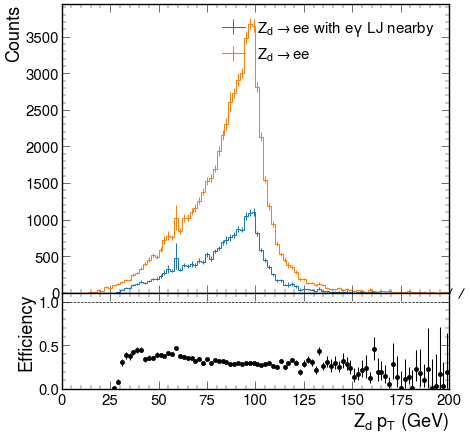
\includegraphics[width = 4cm, height =  4cm]{zd_pt_0.25.png}

\end{column}
\end{columns}
\end{frame}
\begin{frame}{Parameters Considered}

We are considering a wide range of $L_{xy}$, a wide range of lepton $p_T$, and a wide range of lepton collimation, including extremely collimated final states.\\
\vspace{12pt}
Therefore, to get an idea about the LJ reconstruction efficiency in that whole space, we consider the following parameters:
\begin{itemize}
    \item $Z_d$ $p_T$
    \item $Z_d$ $L_{xy}$
    \item $\Delta$R(Leptons)
\end{itemize}
\vspace{12pt}
These variables are highly correlated; we are trying to understand the efficiency while accounting for their correlation.

\end{frame}
\begin{frame}{Lepton Collimation}
\centering
\begin{annotationimage}{width=10cm, height=4cm}{ee_collimation.png}
\draw[coordinate label  = {\textcolor{UniBlue}{$Z_d \rightarrow ee$} at (0.2, -.05)}];
\draw[coordinate label  = {\textcolor{UniBlue}{$Z_d\rightarrow \mu\mu$}  at (0.8, -.05)}];
\end{annotationimage}
\begin{itemize}
    \item Both \textbf{$m_B$} and \textbf{$m_{Z_d}$} affect the collimation of the leptons.
    \item For fixed $m_B$, smallest $m_{Z_d}$ has the highest collimation.
\end{itemize}

\begin{tcolorbox}[colback=uvaorange!5!white,colframe=uvaorange]
\centering
$m_{z_d}$ = 0.25 GeV $\longrightarrow$ More collimated.\\
$m_{z_d}$ = 5 GeV $\longrightarrow$ Less collimated.\\
\end{tcolorbox}
\scriptsize 
To learn more about kinematics, refer to the previous talk's slides  \href{https://indico.cern.ch/event/1319083/}{here} 
\end{frame}
\begin{frame}{}
\centering
\Huge
$e\gamma$ Lepton Jet Reconstruction Efficiency
\end{frame}

\begin{frame}[t]{$Z_d$ $p_T$}

\begin{columns}
\begin{column}{.55\textwidth}
\centering
$L_{xy}<$ 150 cm\\
\scriptsize
\textcolor{UniBlue}{$Z_d\rightarrow ee$}, \textcolor{uvaorange}{$Z_d$ $<L_{xy}>$ = 300 cm}\\
\textcolor{uvaorange}{$m_{Z_d}=$ 0.25 GeV (more collimated)\\}
\begin{annotationimage}{width=3cm, height=3cm}{zd_pt_0.25_lxy150_e.png}
%\draw[coordinate label  = {$Z_d \rightarrow ee$ at (0.5, -.05)}];
%\draw[coordinate label  = {$L_{xy}<150$cm $\downarrow$  at (0.5, 1.1)}];
\end{annotationimage}
\begin{annotationimage}{width=3cm, height=3cm}{1000GeV/zd_ee_pt_0p25_lxyupto150.png}
%\draw[coordinate label  = {\textcolor{UniBlue}{$Z_d \rightarrow ee$} at (0.5, -0.05)}];
%\draw[coordinate label  = {$L_{xy}<150$cm $\downarrow$ at (0.5, 1.1)}];
\end{annotationimage}\\
\textcolor{uvaorange}{$m_{Z_d}=$ 5 GeV (less collimated)\\}
\begin{annotationimage}{width=3cm, height=3cm}{zd_e_pt_5_lxy_150.png}
\draw[coordinate label  = {\textcolor{UniBlue}{$m_{B}=$ 200 GeV} at (0.5, -.05)}];
%\draw[coordinate label  = {$L_{xy}<150$cm $\downarrow$  at (0.5, 1.1)}];
\end{annotationimage}
\begin{annotationimage}{width=3cm, height=3cm}{1000GeV/zd_ee_pt_5_lxyupto150.png}
\draw[coordinate label  = {\textcolor{UniBlue}{$m_B=$ 1000 GeV} at (0.5, -0.05)}];
%\draw[coordinate label  = {$L_{xy}<150$cm $\downarrow$ at (0.5, 1.1)}];
\end{annotationimage}
{\tiny Note: The x ranges are different in these plots}
    
\end{column}
\begin{column}{.45\textwidth}
\normalsize
\begin{itemize}
     \item We see a sharp turn-on at 30 GeV, the cut on $p_T$ we applied on the LJs.
     \vspace{1pt}
     \item For more collimated leptons, efficiency is more or less constant after $p_T >$  30 GeV.
     \vspace{1pt}
     \item  For less collimated leptons, as the $p_T$ increases, the efficiency increases.
     \vspace{1pt}
     \item Overall lower efficiency for the less collimated leptons.
\end{itemize}  
\end{column}
\end{columns}
\end{frame}

\begin{frame}[t]{$Z_d$ $L_{xy}$}

\centering
 $Z_d$ $p_T >$ 30 GeV\\
 
\scriptsize
\textcolor{UniBlue}{$Z_d \rightarrow ee$},
\textcolor{uvaorange}{$m_B$ = 200 GeV, $Z_d$ $<L_{xy}>$ = 300 cm}\\
\centering
\begin{annotationimage}{width=3cm, height=3cm}{zd_ee_lxy_0p25_ptG30.png}
\draw[coordinate label  = {$m_{Z_d}$ = 0.25 GeV at (0.5, -0.05)}];
\end{annotationimage}
\begin{annotationimage}{width=3cm, height=3cm}{zd_ee_lxy_1p2_ptG30.png}
\draw[coordinate label  = {$m_{Z_d}$ = 1.2 GeV at (0.5, -0.05)}];
\end{annotationimage}
\begin{annotationimage}{width=3cm, height=3cm}{zd_ee_lxy_5_ptG30.png}
\draw[coordinate label  = {$m_{Z_d}$ = 5 GeV at (0.5, -0.05)}];
\end{annotationimage}\\
{\tiny \vspace{-9pt}(more collimated) \hspace{5cm} (less collimated)}\\
\small
\vspace{-5pt}
\begin{itemize}
    \item Efficiency extends to the end of ECAL and is basically flat in the more collimated case.
    \item Efficiency in the somewhat displaced region drops as the collimation decreases (reason for overall low efficiency in the less collimated sample).
        \item Current electron ID limits the electron reconstruction to only few cms.
    \item We are good at reconstructing the $Z_d$ decays as photons if the decay happens in ECAL or electrons are more collimated. Other displaced decays are more likely to fail the electron/photon ID.


    \textcolor{red}{}
   %\item With the current iD choices for electron and photon the eletron reconstruction is only relevant before the first tarcker layer( within first few cms). And the photon reconstruction takes over after that. We are always good at reconstructing these decays as photons whne the decay happens in ECAL, but we fail to reconstruct these decays as photons or electrons in the middle regions.
    %Therefore we are studying the how to improve the photon/electron ID.

    \vspace{5pt}
    %\item Overall efficiency is low for highest $m_{Z_d}$. It explains why we saw low efficiency in the $p_T$ plot.
\end{itemize}
\end{frame}

\begin{frame}[t]{ $\Delta$R($e^{gen}_0, e^{gen}_1$)}
\centering
$Z_d$ $p_T >$ 30 GeV, $Z_d$ $L_{xy}<$ 150 cm\\

\scriptsize
\textcolor{UniBlue}{$Z_d \rightarrow ee$},
\textcolor{uvaorange}{$m_B$ = 200 GeV, $Z_d$ $<L_{xy}>$ = 300 cm}\\
\begin{annotationimage}{width=3cm, height=3cm}{genE_genE_dR_ptG30_LxyUpto150_0p25.png}
\draw[coordinate label  = {$m_{Z_d}$ = 0.25 GeV at (0.5, -0.05)}];
\end{annotationimage}
\begin{annotationimage}{width=3cm, height=3cm}{genE_genE_dR_ptG30_LxyUpto150_1p2.png}
\draw[coordinate label  = {$m_{Z_d}$ = 1.2 GeV at (0.5, -0.05)}];
\end{annotationimage}
\begin{annotationimage}{width=3cm, height=3cm}{genE_genE_dR_ptG30_LxyUpto150_5.png}
\draw[coordinate label  = {$m_{Z_d}$ = 5 GeV at (0.5, -0.05)}];
\end{annotationimage}\\
{\tiny \vspace{-8pt}(more collimated) \hspace{5cm} (less collimated)}\\
\normalsize
\begin{itemize}
    \item We see non-zero efficiency in the whole range of $\Delta$R.
     \vspace{1pt}
    \item Efficiency is not changing much as a function of $\Delta$R.
     \vspace{1pt}
    \item Overall lower efficiency for less collimated electrons as we saw earlier in the $L_{xy}$ plot.

\end{itemize}
{\scriptsize Note: The x ranges are different in these plots}


\end{frame}
\begin{frame}[t]{$\Delta$R($e^{gen}_0, e^{gen}_1$) and $Z_d$ $L_{xy}$ }
 \centering
 $Z_d$ $p_T>$ 30 GeV, $Z_d$ $L_{xy}<$ 150 cm\\

 \scriptsize
\textcolor{UniBlue}{$Z_d \rightarrow ee$}, \textcolor{uvaorange}{$m_{Z_d}$ = 1.2 GeV, $m_B$ = 200 GeV, $Z_d$ $<L_{xy}>$ = 300 cm}\\
\centering
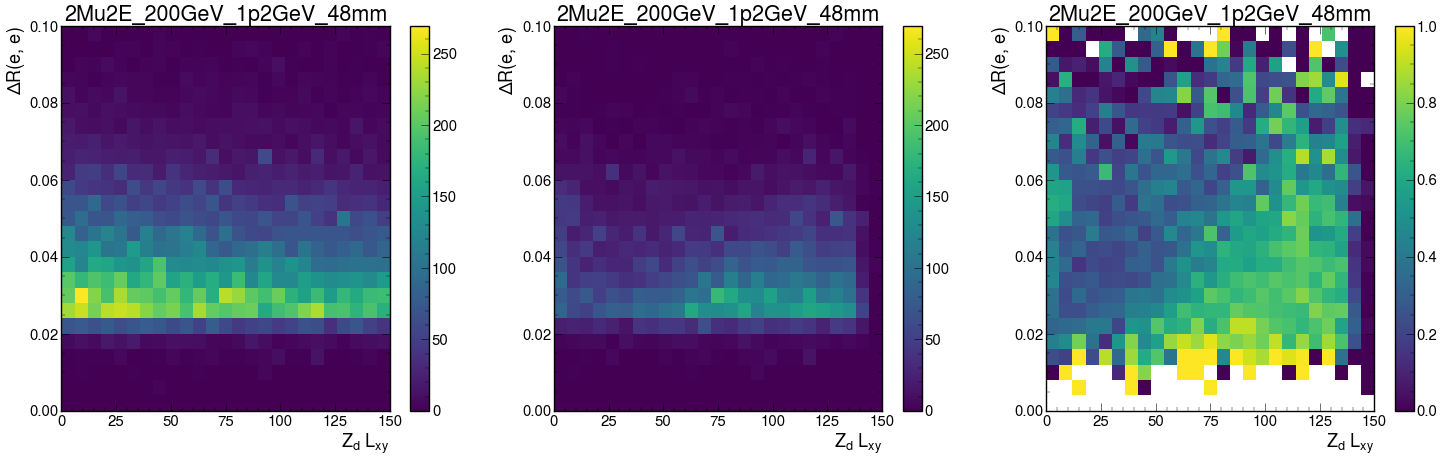
\includegraphics[width =12cm, height =3.5cm]{zd_ee_lxy_dR_1p2.png}\\
{\tiny \textcolor{uvaorange}{\hspace{0cm}den: $Z_d\rightarrow ee$ \hspace{2.5cm } num: $Z_d\rightarrow ee$ with  $e\gamma$ LJ nearby\hspace{2cm} Efficiency\\}}
\normalsize
\begin{itemize}
    \item High efficiency at low $\Delta$R, high $L_{xy}$ Region.
     \vspace{1pt}
    \item If the $L_{xy}$ is bigger than a few cms, we cannot reconstruct them as electrons. If the electrons are too far apart, we fail to identify them as photons.
\end{itemize}
We will try to improve this efficiency by changing the electron/photon ID!
\end{frame}
\begin{frame}{}
\centering
\Huge
$\mu$ Lepton Jet Reconstruction Efficiency
\end{frame}

\begin{frame}[t]{$Z_d$ $p_T$}

\begin{columns}
\begin{column}{.55\textwidth}
\centering
$L_{xy}<$ 400 cm\\
\scriptsize
\textcolor{UniBlue}{$Z_d\rightarrow \mu\mu$}, \textcolor{uvaorange}{$Z_d$ $<L_{xy}>$ = 300 cm}\\
\textcolor{uvaorange}{$m_{Z_d}=$ 0.25 GeV (more collimated)\\}
\begin{annotationimage}{width=3cm, height=3cm}{zd_mu_pt_lxyupto400_0p25.png}
%\draw[coordinate label  = {$Z_d \rightarrow ee$ at (0.5, -.05)}];
%\draw[coordinate label  = {$L_{xy}<150$cm $\downarrow$  at (0.5, 1.1)}];
\end{annotationimage}
\begin{annotationimage}{width=3cm, height=3cm}{1000GeV/zd_mumu_pt_0p25_lxyupto400.png}
%\draw[coordinate label  = {\textcolor{UniBlue}{$Z_d \rightarrow ee$} at (0.5, -0.05)}];
%\draw[coordinate label  = {$L_{xy}<150$cm $\downarrow$ at (0.5, 1.1)}];
\end{annotationimage}\\
\textcolor{uvaorange}{$m_{Z_d}=$ 5 GeV (less collimated)\\}
\begin{annotationimage}{width=3cm, height=3cm}{zd_mu_pt_lxyupto400_5.png}
\draw[coordinate label  = {\textcolor{UniBlue}{$m_{B}=$ 200 GeV} at (0.5, -.05)}];
%\draw[coordinate label  = {$L_{xy}<150$cm $\downarrow$  at (0.5, 1.1)}];
\end{annotationimage}
\begin{annotationimage}{width=3cm, height=3cm}{1000GeV/zd_mumu_pt_5_lxyupto400.png}
\draw[coordinate label  = {\textcolor{UniBlue}{$m_B=$ 1000 GeV} at (0.5, -0.05)}];
%\draw[coordinate label  = {$L_{xy}<150$cm $\downarrow$ at (0.5, 1.1)}];
\end{annotationimage}
{\tiny Note: The x ranges are different in these plots}

    
\end{column}
\begin{column}{.45\textwidth}
\normalsize
\begin{itemize}
  \item We see a sharp turn-on at 30 GeV, the cut on $p_T$ we applied on the LJs.
     \vspace{1pt}
  \item After the turn-on, efficiency slightly decreases as the $p_T$ increases for both cases.
     \vspace{1pt}
  \item Overall lower efficiency at higher $p_T$ for more collimated muons (we suspect it's due the correlation with collimation).
\end{itemize}  
\end{column}
\end{columns}
\end{frame}
\begin{frame}[t]{$Z_d$ $L_{xy}$}
\centering
 $Z_d$ $p_T >$ 30 GeV\\
 \scriptsize
\textcolor{UniBlue}{$Z_d \rightarrow \mu\mu$}, \textcolor{uvaorange}{$m_B$ = 200 GeV, $Z_d$ $<L_{xy}>$ = 300 cm}\\
\centering
\begin{annotationimage}{width=3cm, height=3cm}{zd_mumu_lxy_0p25_ptG30.png}
\draw[coordinate label  = {$m_{Z_d}$ = 0.25 GeV at (0.5, -0.05)}];
\end{annotationimage}
\begin{annotationimage}{width=3cm, height=3cm}{zd_mumu_lxy_1p2_ptG30.png}
\draw[coordinate label  = {$m_{Z_d}$ = 1.2 GeV at (0.5, -0.05)}];
\end{annotationimage}
\begin{annotationimage}{width=3cm, height=3cm}{zd_mumu_lxy_5_ptG30.png}
\draw[coordinate label  = {$m_{Z_d}$ = 5 GeV at (0.5, -0.05)}];
\end{annotationimage}\\
{\tiny \vspace{-9pt}(more collimated) \hspace{5cm} (less collimated)}\\
\normalsize
\begin{itemize}

\item We have efficiency for a wide range of $L_{xy}$.
\vspace{5pt}
\item Efficiency extends to higher $L_{xy}$ for the less collimated muons.
\vspace{5pt}
\item There is a drop in the efficiency at the transition point of PF to DSA for the more collimated sample. We suspect it is due to failure in PF-DSA cross-cleaning/duplicate removal.

\end{itemize}
\end{frame}
\begin{frame}[t]{ $\Delta$R($\mu^{gen}_0, \mu^{gen}_1$)}
\centering
$Z_d$ $p_T >$ 30 GeV, $Z_d$ $L_{xy}<$ 400 cm\\
\scriptsize
\textcolor{UniBlue}{$Z_d \rightarrow \mu\mu$}, \textcolor{uvaorange}{$m_B$ = 200 GeV, $Z_d$ $<L_{xy}>$ = 300 cm}\\
\begin{annotationimage}{width=3cm, height=3cm}{genMu_genMu_dR_ptG30_LxyUpto400_0p25.png}
\draw[coordinate label  = {$m_{Z_d}$ = 0.25 GeV at (0.5, -0.05)}];
\end{annotationimage}
\begin{annotationimage}{width=3cm, height=3cm}{genMu_genMu_dR_ptG30_LxyUpto400_1p2.png}
\draw[coordinate label  = {$m_{Z_d}$ = 1.2 GeV at (0.5, -0.05)}];
\end{annotationimage}
\begin{annotationimage}{width=3cm, height=3cm}{genMu_genMu_dR_ptG30_LxyUpto400_5.png}
\draw[coordinate label  = {$m_{Z_d}$ = 5 GeV at (0.5, -0.05)}];
\end{annotationimage}\\
{\tiny \vspace{-9pt}(more collimated) \hspace{5cm} (less collimated)}\\
\normalsize
\begin{itemize}
    \item We see non-zero efficiency in the entire range of $\Delta$R.
    \vspace{5pt}
    \item No strong dependence on $\Delta$R, but interesting trend which we can explore more through 2D Efficiency.
\end{itemize}
{\scriptsize Note: The x ranges are different in these plots}
\end{frame}

\begin{frame}[t]{$\Delta$R($\mu^{gen}_0, \mu^{gen}_1$) and $Z_d$ $L_{xy}$ }
\centering
$Z_d$ $p_T>$ 30 GeV, $Z_d$ $L_{xy}<$ 400 cm\\
\scriptsize
\textcolor{UniBlue}{$Z_d \rightarrow \mu\mu$}, \textcolor{uvaorange}{$m_{Z_d}$ = 5 GeV,$m_B$ = 200 GeV, $Z_d$ $<L_{xy}>$ = 300 cm}\\
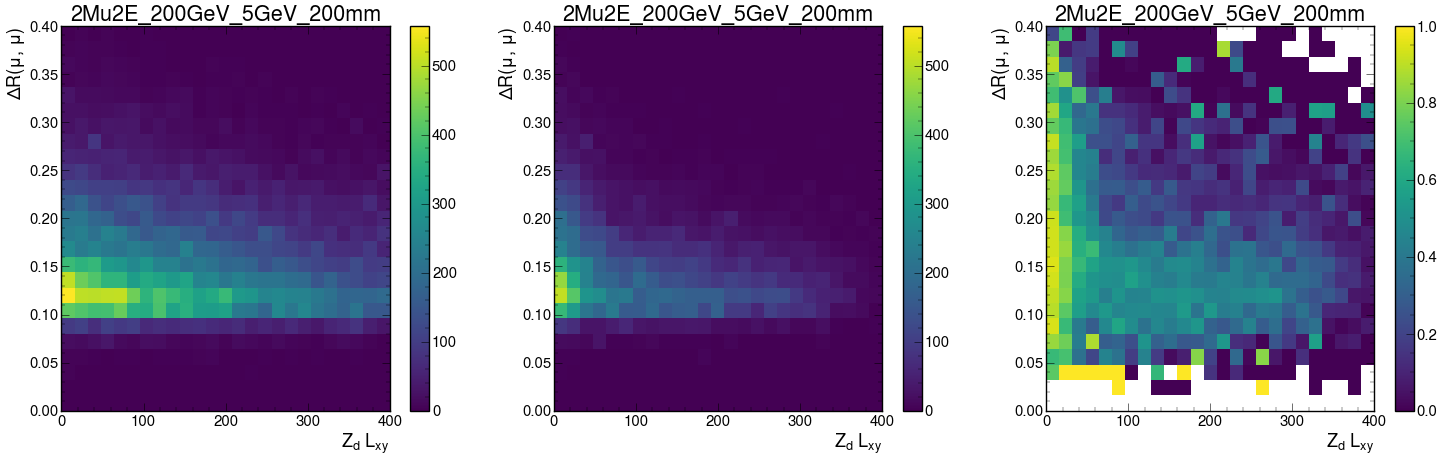
\includegraphics[width =12cm, height =3.5cm]{zd_mumu_lxy_dR_5.png}\\
{\tiny \textcolor{uvaorange}{\hspace{-1cm}den: $Z_d\rightarrow\mu\mu$ \hspace{2.5cm } num: $Z_d\rightarrow\mu\mu$ with  $\mu$ LJ nearby\hspace{2cm} Efficiency\\}}

\normalsize
\begin{itemize}
    \item Overall high efficiency for low $L_{xy}$ region.
     \vspace{1pt}
    \item At higher $L_{xy}$, the efficiency falls as $\Delta$R increases (DSA muon region).
     \vspace{1pt}
    \item This is totally counterintuitive; we expect muon reconstruction to be easier at higher $\Delta$R and thereby high efficiency. 

\end{itemize}
 We can look at this again with another variable $Z_d$ $p_T$!
\end{frame}

\begin{frame}[t]{$\Delta$R($\mu^{gen}_0, \mu^{gen}_1$) and $Z_d$ $p_T$ }
\centering
$Z_d$ $p_T>$ 30 GeV, $Z_d$ $L_{xy}<$ 400 cm\\
\scriptsize
\textcolor{UniBlue}{$Z_d \rightarrow \mu\mu$}, \textcolor{uvaorange}{$m_{Z_d}$ = 5 GeV,$m_B$ = 200 GeV, $Z_d$ $<L_{xy}>$ = 300 cm}\\
\centering
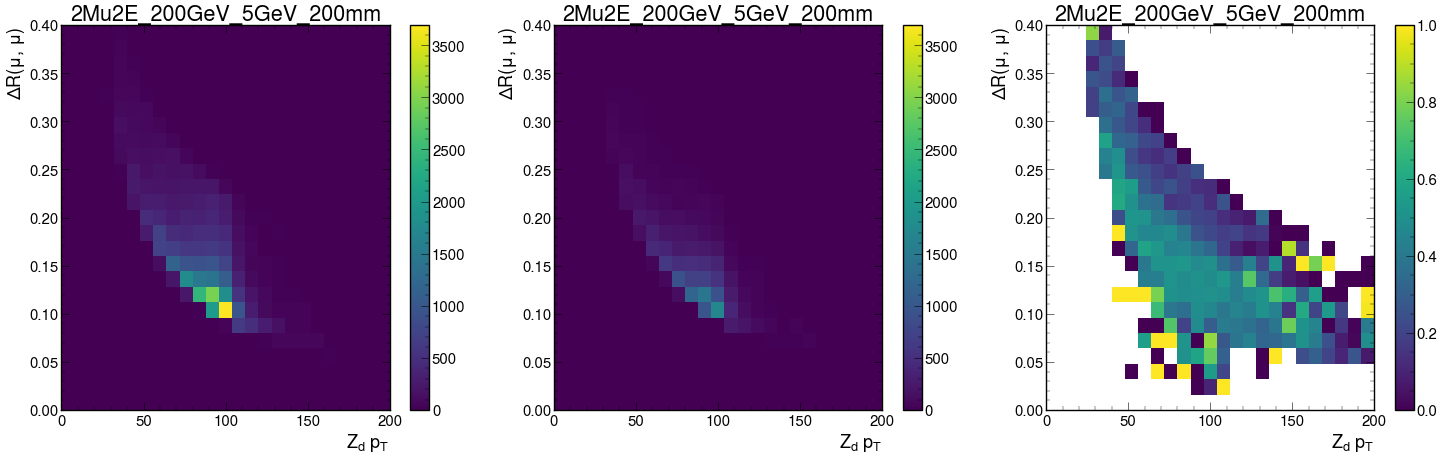
\includegraphics[width =12cm, height =3.5cm]{zd_mumu_pt_dR_5.png}\\
{\tiny \textcolor{uvaorange}{\hspace{-1cm}den: $Z_d\rightarrow\mu\mu$ \hspace{2.5cm } num: $Z_d\rightarrow\mu\mu$ with  $\mu$ LJ nearby\hspace{2cm} Efficiency\\}}

\normalsize
\begin{itemize}
\item  Overall high efficiency in low $\Delta$R region.
     \vspace{1pt}
\item For a fixed $p_T$, low efficiency for higher $\Delta$R region.
\end{itemize}
We need to study the higher $\Delta$R region more!
\end{frame}


\begin{frame}{Looking at PF-PF, PF-DSA, DSA-DSA Separately}
\framesubtitle{$\Delta$R($\mu^{gen}_0, \mu^{gen}_1$) and $\mu_0^{gen}$ $p_T$ }
\footnotesize
\begin{columns}
\begin{column}{.7\textwidth}
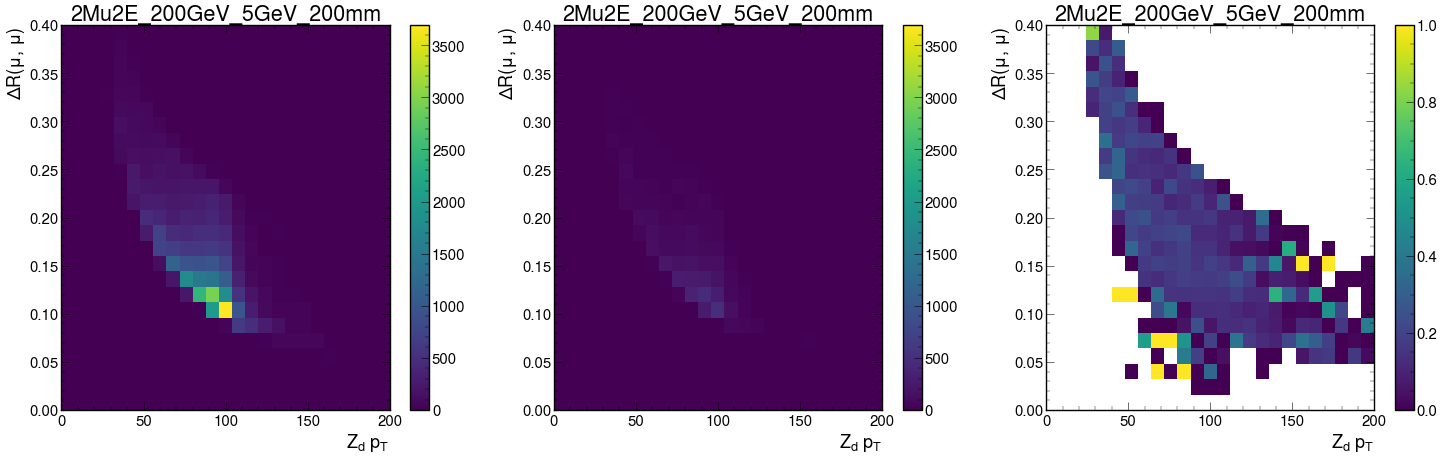
\includegraphics[width =8cm, height =2cm]{zd_mumu_pt_dR_5_pf.png}\\

\end{column}
\begin{column}{.3\textwidth}
\textcolor{UniBlue}{PF-PF:} No strong dependence on $\Delta$R.
\end{column}
\end{columns}

\begin{columns}
\begin{column}{.7\textwidth}
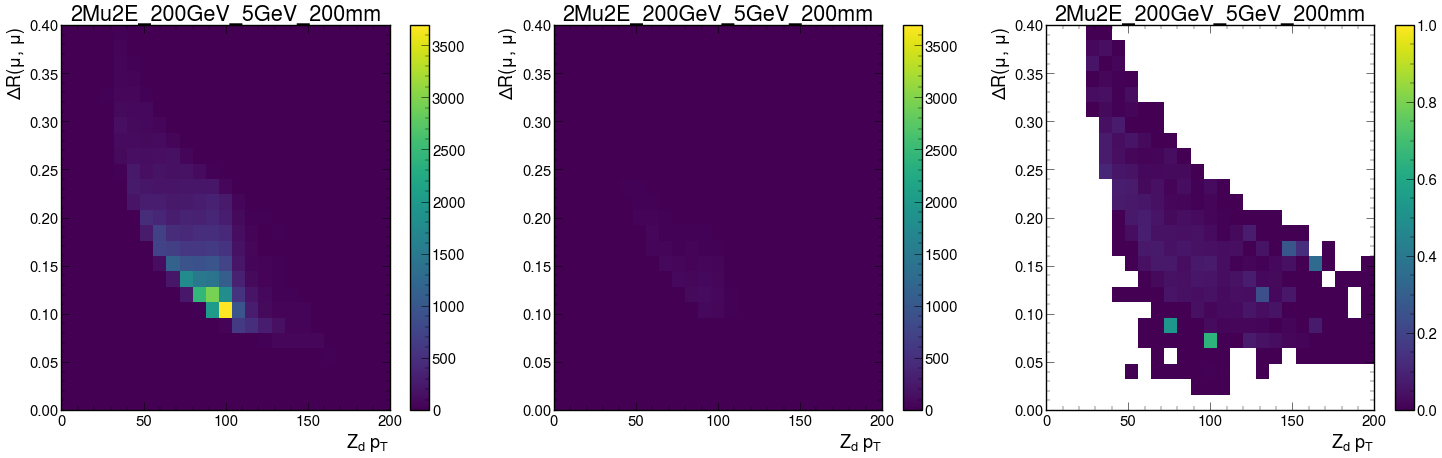
\includegraphics[width =8cm, height =2cm]{zd_mumu_pt_dR_5_1dsa1pf.png}\\
\end{column}
\begin{column}{.3\textwidth}
\textcolor{UniBlue}{PF-DSA:} Not strong dependence on $\Delta$R.
\end{column}
\end{columns}
\begin{columns}
\begin{column}{.7\textwidth}
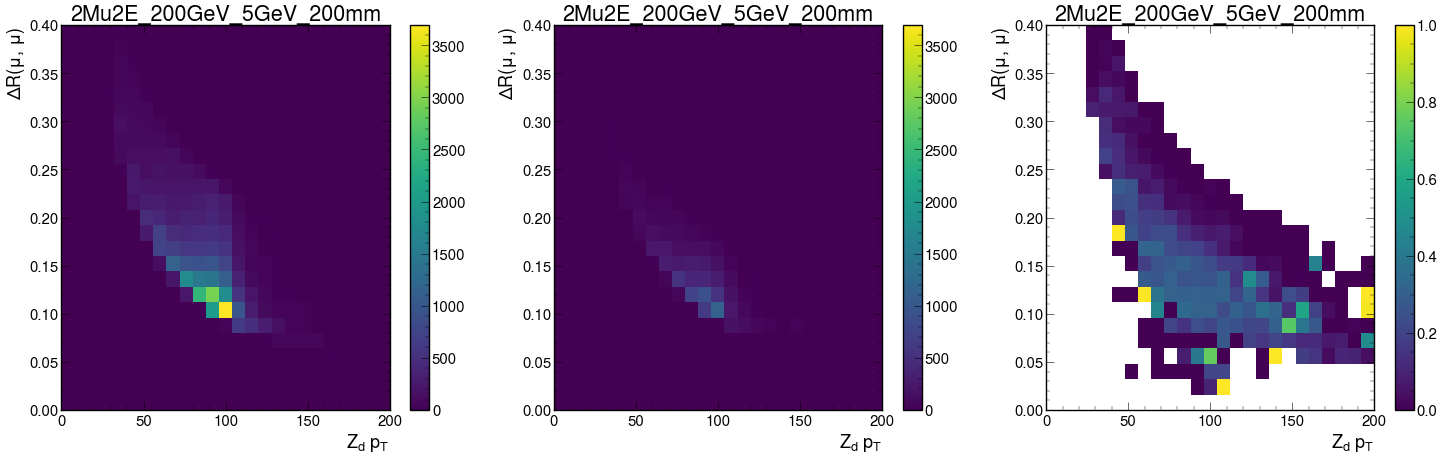
\includegraphics[width =8cm, height =2cm]{zd_mumu_pt_dR_5_2dsa.png}\\
\end{column}
\begin{column}{.3\textwidth}
\textcolor{UniBlue}{DSA-DSA:} For a given $p_T$, efficiency falls as $\Delta$R increases.
\end{column}
\end{columns}
{\tiny \textcolor{uvaorange}{\hspace{12pt}den: $Z_d\rightarrow\mu\mu$ \hspace{25pt } num: $Z_d\rightarrow\mu\mu$ with \hspace{1cm} Efficiency\\
\vspace{-5pt}
\hspace{ 3cm } $\mu$ LJ nearby}}

We need to study the DSA-DSA $\mu$-type LJs more!

\end{frame}
\begin{frame}[t]{$\Delta$R($\mu^{gen}_0, \mu^{gen}_1$) and $\mu_1^{gen}$ $p_T$ }
\centering
\textcolor{red}{Looking at only DSA-DSA $\mu$ LJs}\\
 $Z_d$ $p_T>$ 30 GeV, $Z_d$ $L_{xy}<$ 400 cm\\
 \scriptsize
\textcolor{UniBlue}{$Z_d \rightarrow \mu\mu$},\textcolor{uvaorange}{$m_{Z_d}$ = 5 GeV,$m_B$ = 200 GeV, $Z_d$ $<L_{xy}>$ = 300 cm}\\
\centering
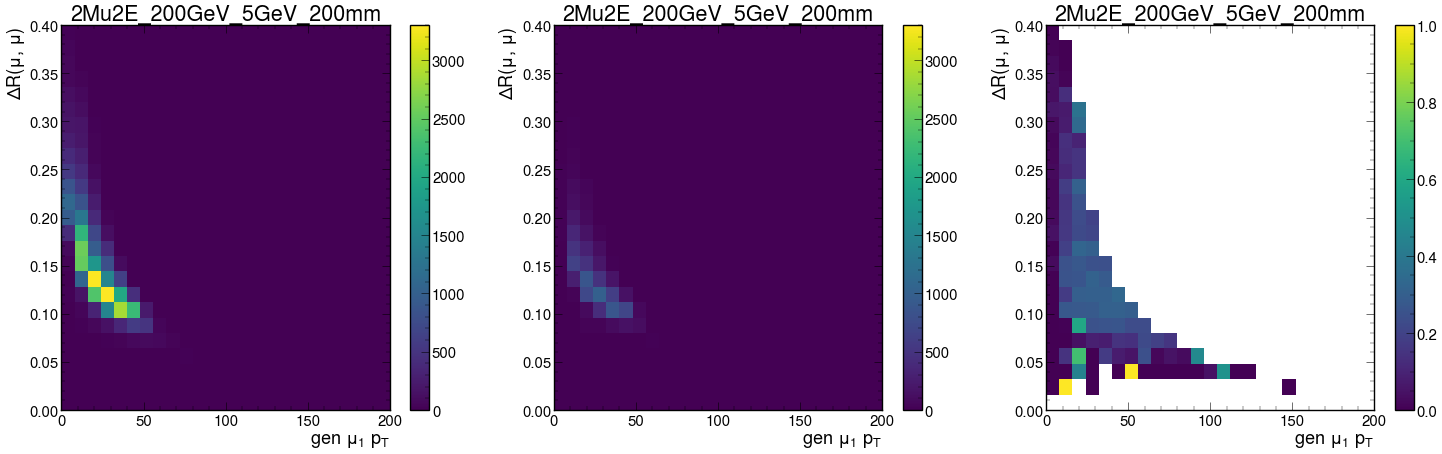
\includegraphics[width =12cm, height =3.5cm]{zd_mumu_genMu1_pt_dR_5_2dsa.png}\\
{\tiny \textcolor{uvaorange}{\hspace{-1cm}den: $Z_d\rightarrow\mu\mu$ \hspace{2.5cm } num: $Z_d\rightarrow\mu\mu$ with  $\mu$ LJ nearby\hspace{2cm} Efficiency\\}}

\normalsize
\begin{itemize}
\item Low efficiency is concentrated in the low sub-leading muon pT region.
     \vspace{1pt}
\item High $\Delta$R corresponds to low sub-leading $p_T$.
\end{itemize}
We check whether it is true for a fixed leading $\mu$ $p_T$.
\end{frame}


\begin{frame}[t]{Applying Cut On Leading $\mu$ $p_T$}
\framesubtitle{$\Delta$R($\mu^{gen}_0, \mu^{gen}_1$) and $\mu_1^{gen}$ $p_T$}

\centering
\textcolor{red}{Looking at DSA-DSA $\mu$ LJ}\\
 $Z_d$ $p_T>$ 30 GeV, $Z_d$ $L_{xy}<$ 150 cm, 50  $<= \mu_0^{gen}$ $p_T<=$ 60 GeV\\
\scriptsize
\textcolor{UniBlue}{$Z_d \rightarrow \mu\mu$}, \textcolor{uvaorange}{$m_{Z_d}$ = 5 GeV,$m_B$ = 200 GeV, $Z_d$ $<L_{xy}>$ = 300 cm}\\
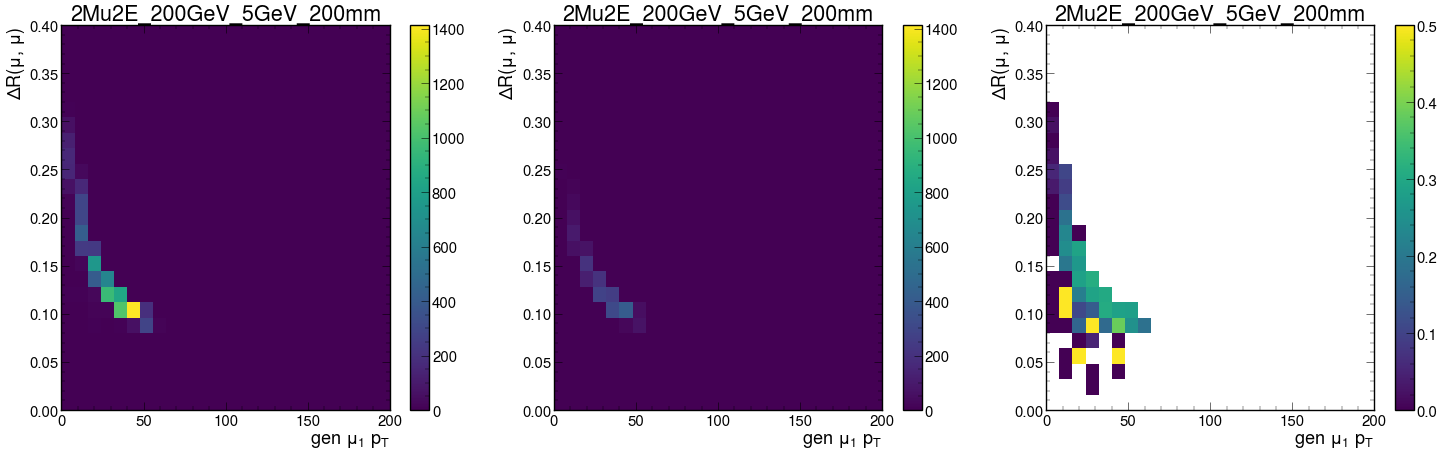
\includegraphics[width =12cm, height =3.5cm]{zd_mumu_genMu1_pt_dR_5_leadingpT_50to60.png}\\
{\tiny \textcolor{uvaorange}{\hspace{-1cm}den: $Z_d\rightarrow\mu\mu$ \hspace{2.5cm } num: $Z_d\rightarrow\mu\mu$ with  $\mu$ LJ nearby\hspace{2cm} Efficiency\\}}
\normalsize
\begin{itemize}
    \item  We observe that the high $\Delta$R corresponds to low sub-leading $p_T$. And the lower $p_T$ muons don't pass our 10GeV cut.
\end{itemize}

    
\end{frame}

\begin{frame}{Conclusion}
 We see good efficiency in a large range of the parameter space we are considering.\\
\textbf{For $Z_d \rightarrow ee$ ($e\gamma$ LJ):}\\
\begin{itemize}
\item No serious dependence on $p_T$ for both more collimated and less collimated electrons
\item We see behaviours which depend on the collimation of the electrons. In the most collimated case, we are really good at reconstructing at all displacements. We see low efficiency in the somewhat displaced region (decay in the tracker) when the electrons are less collimated. 
\item We are actively investigating how to improve the electron/photon ID to recover efficiency.

\end{itemize}
\textbf{For $Z_d\rightarrow \mu\mu$ ($\mu$ LJ):}\\
\begin{itemize}
\item Efficiency extends out to very high displacements, even for extremely collimated muon pairs. 
\item We see a drop in efficiency in the higher $\Delta$R regions, as the higher $\Delta$R regions corresponds to the low sub-leading $\mu$ $p_T$ and they fail to pass the cuts applied.
\end{itemize}
\end{frame}
\begin{frame}{}
\centering
\Huge
THANK YOU
\end{frame}
\begin{frame}[noframenumbering]{}
\centering
\Huge
BACK UP
\end{frame}
\begin{frame}[noframenumbering,t]{Separating the $e\gamma$ LJs}
\framesubtitle{$Z_d$ $L_{xy}$}
\centering \textcolor{UniBlue}{$e$ -type}: $N_e >$ 0\\
\begin{annotationimage}{width=3cm, height=3cm}{zd_mumu_lxy_0p25_ptG30_eLj.png}
%\draw[coordinate label  = {$m_{Z_d}$ = 0.25 GeV at (0.5, -0.05)}];
\end{annotationimage}
\begin{annotationimage}{width=3cm, height=3cm}{zd_mumu_lxy_1p2_ptG30_eLj.png}
%\draw[coordinate label  = {$m_{Z_d}$ = 0.25 GeV at (0.5, -0.05)}];
\end{annotationimage}
\begin{annotationimage}{width=3cm, height=3cm}{zd_mumu_lxy_5_ptG30_eLj.png}
%\draw[coordinate label  = {$m_{Z_d}$ = 0.25 GeV at (0.5, -0.05)}];
\end{annotationimage}\\


\textcolor{UniBlue}{$\gamma$ -type: }$N_{\gamma}>$0, $N_e=$ 0\\
\begin{annotationimage}{width=3cm, height=3cm}{zd_mumu_lxy_0p25_ptG30_gLj.png}
\draw[coordinate label  = {$m_{Z_d}$ = 0.25 GeV at (0.5, -0.05)}];
\end{annotationimage}
\begin{annotationimage}{width=3cm, height=3cm}{zd_mumu_lxy_1p2_ptG30_gLj.png}
\draw[coordinate label  = {$m_{Z_d}$ = 1.2 GeV at (0.5, -0.05)}];
\end{annotationimage}
\begin{annotationimage}{width=3cm, height=3cm}{zd_mumu_lxy_5_ptG30_gLj.png}
\draw[coordinate label  = {$m_{Z_d}$ = 5 GeV at (0.5, -0.05)}];
\end{annotationimage}\\
\end{frame}
\begin{frame}[noframenumbering,t]{$\Delta$R($e^{gen}_0, e^{gen}_1$) and $Z_d$ $p_T$ }
\centering
$Z_d$ $p_T>$ 30 GeV, $Z_d$ $L_{xy}<$ 150 cm\\
\scriptsize
\textcolor{UniBlue}{$Z_d \rightarrow ee$}, \textcolor{uvaorange}{$m_{Z_d}$ = 1.2 GeV,$m_B$ = 200 GeV, $Z_d$ $<L_{xy}>$ = 300 cm}\\
\centering
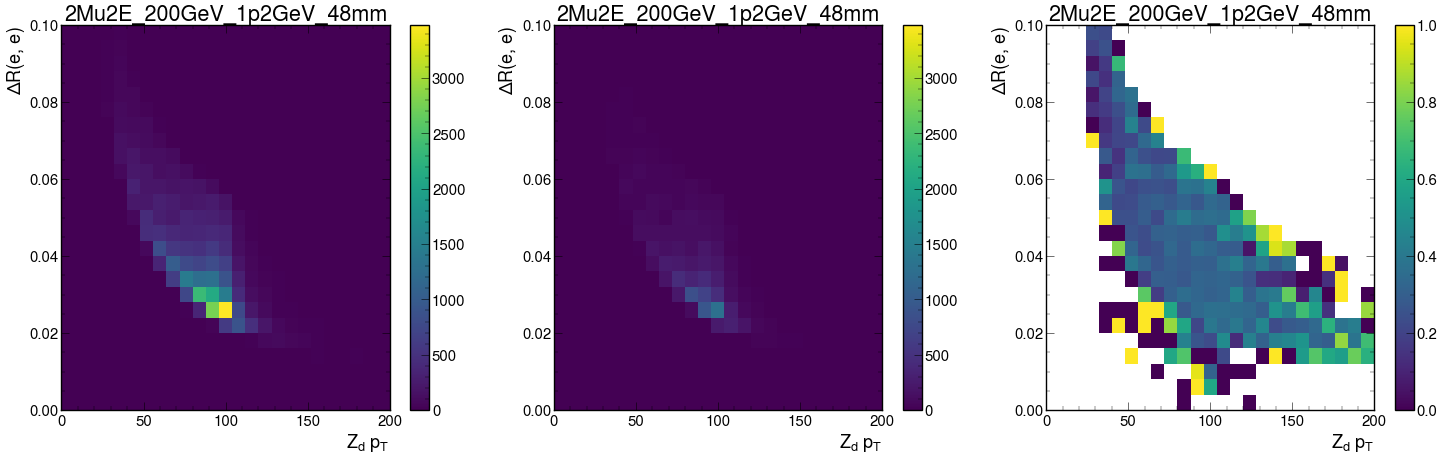
\includegraphics[width =12cm, height =3.5cm]{zd_ee_pt_dR_1p2.png}\\
{\tiny \textcolor{uvaorange}{\hspace{-1cm}den: $Z_d\rightarrow ee$ \hspace{2.5cm } num: $Z_d\rightarrow ee$ with  $e\gamma$ LJ nearby\hspace{2cm} Efficiency\\}}
\normalsize
\begin{itemize}
    \item Efficiency doesn't have a huge change in the range shown.
\end{itemize}
    
\end{frame}
\begin{frame}[noframenumbering,t]{ $Z_d$ $L_{xy}$ and $Z_d$ $p_T$ }
\centering
$Z_d$ $p_T>$ 30 GeV, $Z_d$ $L_{xy}<$ 150 cm\\
\scriptsize
\textcolor{UniBlue}{$Z_d \rightarrow ee$}, \textcolor{uvaorange}{$m_{Z_d}$ = 1.2 GeV,$m_B$ = 200 GeV, $Z_d$ $<L_{xy}>$ = 300 cm}\\
\centering
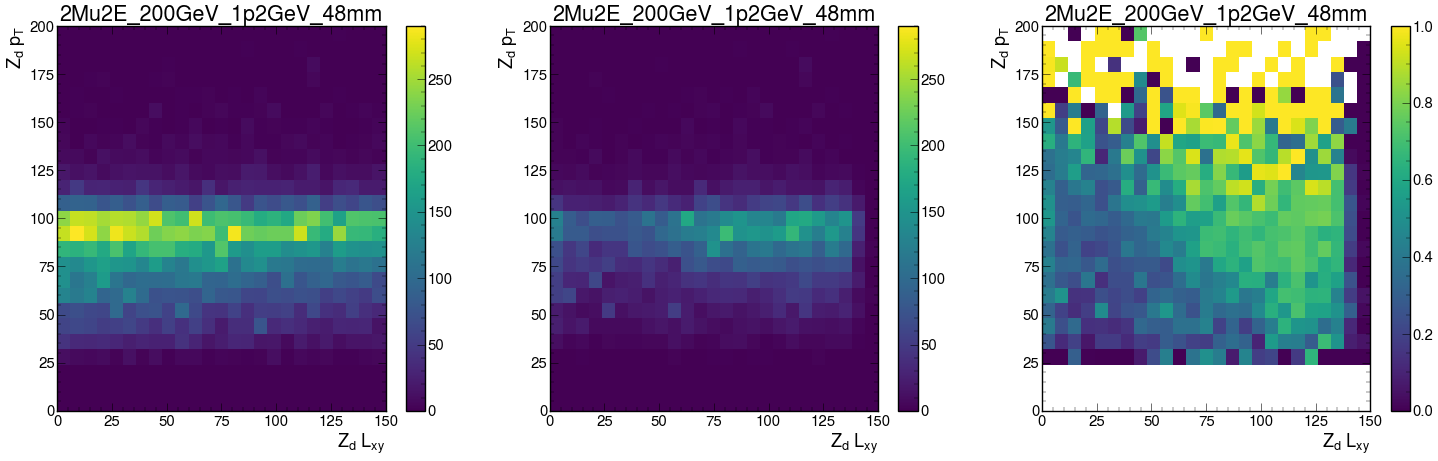
\includegraphics[width =12cm, height =3.5cm]{zd_ee_lxy_pT_1p2.png}\\
{\tiny \textcolor{uvaorange}{\hspace{-1cm}den: $Z_d\rightarrow ee$ \hspace{2.5cm } num: $Z_d\rightarrow e e$ with  $e\gamma$ LJ nearby\hspace{2cm} Efficiency\\}}
\normalsize
\begin{itemize}
    \item High Efficiency at high $p_T$ and high $L_{xy}$ region.
    \item Very low efficiency for low $L_{xy}$ and low $p_T$. 
    \item The correlation between $L_{xy}$ and $p_T$ is something we already saw before.
\end{itemize}
\end{frame}

\begin{frame}[noframenumbering]{Separating the $\mu$ LJs}
\framesubtitle{$Z_d$ $L_{xy}$}
\centering \textcolor{UniBlue}{PF$\mu$ -type} : $N_{DSA} =$ 0\\
\begin{annotationimage}{width=3cm, height=3cm}{zd_mumu_lxy_0p25_ptG30_pfMuLj.png}
%\draw[coordinate label  = {$m_{Z_d}$ = 0.25 GeV at (0.5, -0.05)}];
\end{annotationimage}
\begin{annotationimage}{width=3cm, height=3cm}{zd_mumu_lxy_1p2_ptG30_pfMuLj.png}
%\draw[coordinate label  = {$m_{Z_d}$ = 0.25 GeV at (0.5, -0.05)}];
\end{annotationimage}
\begin{annotationimage}{width=3cm, height=3cm}{zd_mumu_lxy_5_ptG30_pfMuLj.png}
%\draw[coordinate label  = {$m_{Z_d}$ = 0.25 GeV at (0.5, -0.05)}];
\end{annotationimage}\\


\textcolor{UniBlue}{DSA $\mu$ -type:} $N_{DSA}>$0\\
\begin{annotationimage}{width=3cm, height=3cm}{zd_mumu_lxy_0p25_ptG30_dsaMuLj.png}
\draw[coordinate label  = {$m_{Z_d}$ = 0.25 GeV at (0.5, -0.05)}];
\end{annotationimage}
\begin{annotationimage}{width=3cm, height=3cm}{zd_mumu_lxy_1p2_ptG30_dsaMuLj.png}
\draw[coordinate label  = {$m_{Z_d}$ = 1.2 GeV at (0.5, -0.05)}];
\end{annotationimage}
\begin{annotationimage}{width=3cm, height=3cm}{zd_mumu_lxy_5_ptG30_dsaMuLj.png}
\draw[coordinate label  = {$m_{Z_d}$ = 5 GeV at (0.5, -0.05)}];
\end{annotationimage}\\
    
\end{frame}
\begin{frame}[noframenumbering,t]{LJ Reconstruction Efficiency w.r.t \\  $Z_d$ $L_{xy}$ and $Z_d$ $p_T$ }
\centering
$Z_d$ $p_T>$ 30 GeV, $Z_d$ $L_{xy}<$ 400 cm\\
\scriptsize
\textcolor{UniBlue}{$Z_d \rightarrow \mu\mu$}, \textcolor{uvaorange}{$m_{Z_d}$ = 5 GeV,$m_B$ = 200 GeV, $Z_d$ $<L_{xy}>$ = 300 cm}\\
\centering
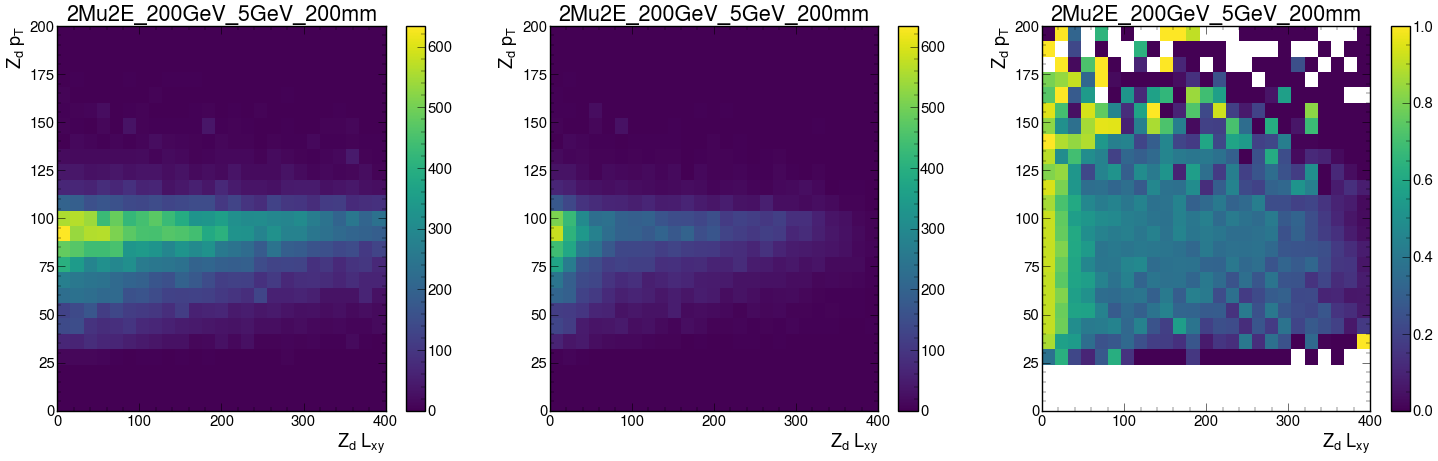
\includegraphics[width =12cm, height =3.5cm]{zd_mumu_lxy_pt_5.png}\\
{\tiny \textcolor{uvaorange}{\hspace{-1cm}den: $Z_d\rightarrow\mu\mu$ \hspace{2.5cm } num: $Z_d\rightarrow\mu\mu$ with  $\mu$ LJ nearby\hspace{2cm} Efficiency\\}}
\normalsize
\begin{itemize}
    \item High Efficiency for low $L_{xy}$ regions.
    \item For a fixed $p_T$, low $L_{xy}$ region show high efficiency.
    \item For a fixed $L_{xy}$, $p_T$ is not varying that much.
\end{itemize}
\end{frame}

\begin{frame}[noframenumbering,t]{$\Delta$R($\mu^{gen}_0, \mu^{gen}_1$) and $\mu_0^{gen}/\mu_1^{gen}$ $p_T$ }
\centering
 $Z_d$ $p_T>$ 30 GeV, $Z_d$ $L_{xy}<$ 400 cm\\
 \scriptsize
\textcolor{UniBlue}{$Z_d \rightarrow \mu\mu$}, \textcolor{uvaorange}{$m_{Z_d}$ = 5 GeV,$m_B$ = 200 GeV, $Z_d$ $<L_{xy}>$ = 300 cm}\\
\centering
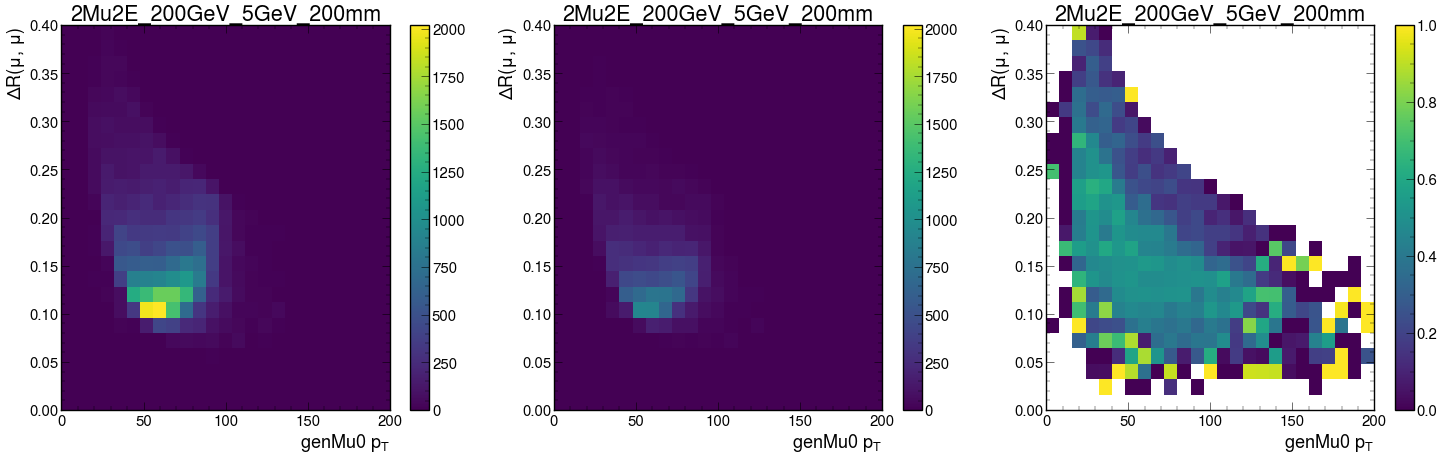
\includegraphics[width =8cm, height =2.5cm]{zd_mumu_genMu0_pt_dR_5.png}\\
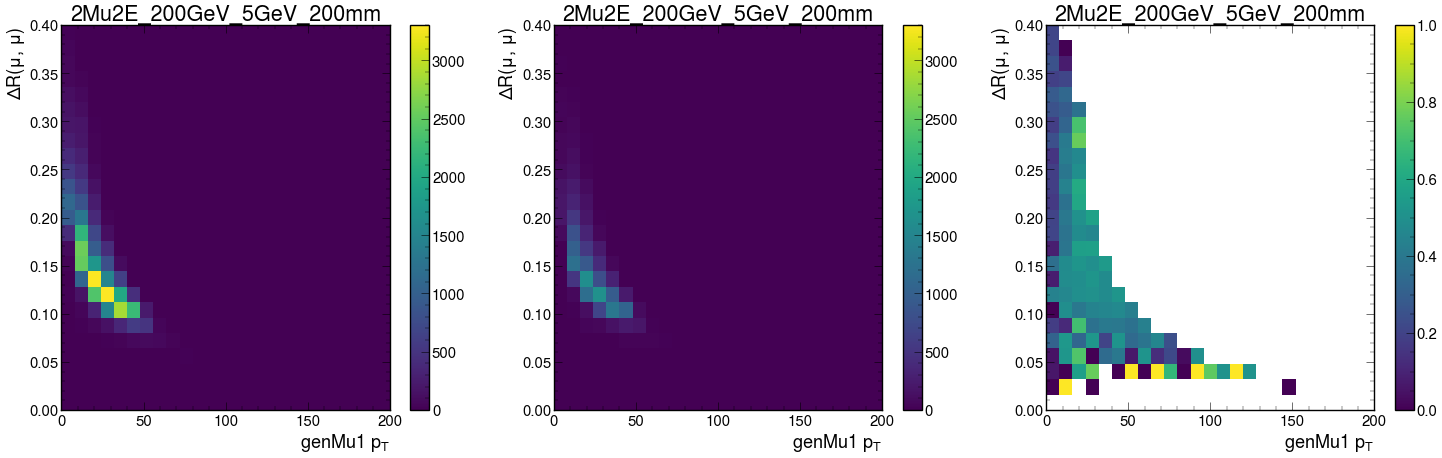
\includegraphics[width =8cm, height =2.5cm]{zd_mumu_genMu1_pt_dR_5.png}\\
{\tiny \textcolor{uvaorange}{den: $Z_d\rightarrow\mu\mu$ \hspace{36pt} num: $Z_d\rightarrow\mu\mu$ with \hspace{36pt} Efficiency\\
\vspace{-5pt}
\hspace{ 1cm } $\mu$ LJ nearby}}
\end{frame}
\begin{frame}[noframenumbering,t]{ $Z_d$ $p_T$ and $\Delta$R($e_0^{gen}$, $e_1^{gen}$) }
\centering
$Z_d$ $p_T>$ 30 GeV, $Z_d$ $L_{xy}<$ 150 cm\\
\scriptsize
\textcolor{UniBlue}{$Z_d \rightarrow \mu\mu$}, \textcolor{uvaorange}{$m_{Z_d}$ = 1.2 GeV,$m_B$ = 200 GeV, $Z_d$ $<L_{xy}>$ = 300 cm}\\
\centering
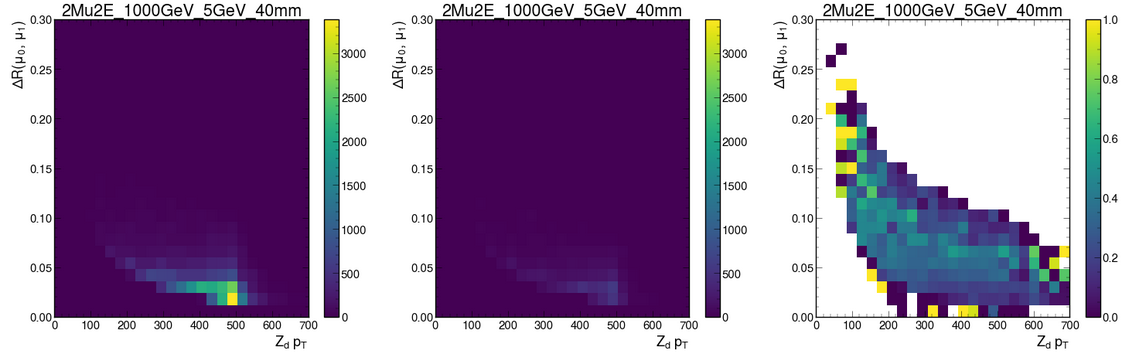
\includegraphics[width =12cm, height =3.5cm]{image (15).png}\\
{\tiny \textcolor{uvaorange}{\hspace{-1cm}den: $Z_d\rightarrow\mu\mu$ \hspace{2.5cm } num: $Z_d\rightarrow\mu\mu$ with  $\mu$ LJ nearby\hspace{2cm} Efficiency\\}}
\normalsize

\end{frame}

%\begin{frame}{References}
%\printbibliography[heading=none]
%\end{frame}
\end{document}